\documentclass[a4paper,8pt]{article}
\usepackage[utf8]{inputenc}
\usepackage[bitstream-charter]{mathdesign}
\usepackage{ragged2e}
\usepackage{anysize}%Paquete que permite cambiar márgenes
\marginsize{1cm}{1cm}{2cm}{2cm}
\usepackage{amsmath}%Paquete para insertar símbolos matemáticos
\usepackage{hyperref}%Paquete para insertar referencias en el texto
\usepackage{textcomp,gensymb}
\usepackage{float}%Paquete para tratar figuras y tablas como flotantes
\usepackage{lipsum}%Paquete para insertar texto mudo
\usepackage{graphicx}
\usepackage{caption}
\usepackage{subcaption}
\usepackage{array}
\usepackage{url}%Paquete para insertar URL's
\usepackage{multicol}%Paquete para crear ambientes multicolumna
\setlength\columnsep{18pt}%Especifíca separación de las columnas
\renewenvironment{abstract}%Modifica el ambientes abstract para modificar la alineación
\usepackage{csquotes}
\usepackage{booktabs} % For better-looking tables
\usepackage{array} % For custom column widths
\usepackage{amsmath} % For mathematical symbols
\hypersetup{
    colorlinks=true,
    linkcolor=black,
    urlcolor=blue,
    citecolor=black
}


\usepackage{geometry}
\usepackage{amsmath} % for equation environment
\usepackage{csquotes}

\geometry{left=1.5cm, right = 1cm, top=2cm,bottom=2.4cm}

\title{INFORME X}
%-----------------------------------------------------------------------------------------------------------------------------------------
\usepackage{biblatex}
\addbibresource{ref.bib}

\bibliography{ref}

\begin{document}

\begin{center}
\Huge{Cluster algorithms}
\vspace{0.4cm}

\normalsize
\large{Devashish Tiwari (20097) and Akshey Rajoriya (2310503)} \\
\vspace{0.06cm}
\textit{\small{}\\
\large{Computational Physics Project}}\\
\small{}
\end{center}


\section{Introduction}

The 2D Ising model stands as a momentous model in physics, showcasing a genuine phase transition. It was solved exactly by Ernst Ising (1D) in 1920 and in 2D analytically solved by Onsager(2D) \supercite{PhysRev.65.117} in 1944. We here present the methods to solve Ising model using three different approaches. Due to its lack of intrinsic dynamical evolution, its simulation relies on Monte Carlo algorithms. Particularly near its phase transition, the Metropolis algorithm's efficiency declines sharply, a limitation circumvented by the SW and Wolff method. Critical exponents describe this phase transition, their determination and comparison to theoretical values form the bases of this report. Finally, the performance of all three algorithms is compared. We then apply the use of these cluster algorithms to Hard sphere model, and presented its comparison with theoritical description, concluding this study which is conducted as part of the Computational Physics course (PHY612N) taught by Dr. Sunil Pratap Singh at the Department of Physics, IISER Bhopal.


\section{Ising model}
Ising model or the Heisenberg model describes the ferromagnetic interaction between the neighbouring spins by the given hamiltonian,
\begin{equation}
    H = - J_{ij} \underset{i,j}{\sum} \sigma_{i} \sigma_{j} - h \underset{i}{\sum} \sigma_{i}
\end{equation}
where $J_{ij}$ is the interaction strength (or spin coupling constant) and is non-zero only for the nearest neighbours. The spins have only two possible orientations along a chosen axis \enquote{up} (+1) or \enquote{down} (-1). and h is the magnetic field strength. There is also a plethora of other physical situations that can be mapped onto Ising models with various forms of the interaction $J_{ij}$ and the field h in binary alloys (where $\sigma_{i}$ correspond to the two species of atoms) and atoms adsorbed on surfaces (where $\sigma_{i}$ correspond to the presence of absence of an atom on a surface).

\vspace{0.2cm}
\noindent Ising found the solution to this problem for a 1D lattice (‘einfache lineare Kette’). The solution to the 2D Ising model for a zero magnetic field was found by L. Onsager. He saw that
there was a phase transition present characterised by the vanishing of the magnetisation of the system. The 3D model still unsolved analytically stands as the numerically solved model with a similar phase transitions. \\

\noindent In our case, we will simulate the model in 2D for zero magnetic field. \\
\begin{equation}
    H = -J_{ij} \underset{i,j}{\sum} \sigma_{i} \sigma_{j} \label{eq:hamiltonian}
\end{equation}

\section{Phase Transitions}
The 2D Ising model has a second order phase transition from a magnetic (ordered) phase to a nonmagnetic (disordered) phase for which the average magnetisation is nonzero and zero, respectively. The temperature at which this transition occurs is the called critical temperature $T_c$. The exact solution by Onsager, shows:
\begin{equation}
    \mathrm{Sinh} (J \beta) \mathrm{Sinh} (J' \beta) = 1,
\end{equation}
where $J$ and $J'$ are spin coupling constant in x and y direction respectively and $\beta = \frac{1}{k_B T_c}$. In this project, we kept the coupling to be constant(=1) in both the perpendicular directions, and thus, $K_B T_c$ in units of J was calculated to be:
\begin{equation}
    T_c = \frac{2}{ln(1 + 2 \sqrt(2)}
\end{equation}

\subsection{Critical exponents}
In the neighbourhood of the critical temperature the thermodynamic quantities(TDQ) show a behaviour
which can be described by so-called critical exponents\supercite{baxter1982exactly}. These exponents theoretically calculated for Ising model are shown in table 1.

\begin{table}[htbp]
    \centering
    \label{tab:tdq_critical_exponents}
    \begin{tabular}{l|l}
    \hline
    \textbf{Relations of TDQ} & \textbf{Critical Exponent} \\
    \hline
    $c_v(T) \propto |T-T_c|^{-\alpha}$ & $\alpha=0$ \\
    $m(T) \propto (T_c-T)^\beta, T<T_c$ & $\beta=\frac{1}{8}$ \\
    $\chi(T) \propto |T-T_c|^{-\gamma}$ & $\gamma=\frac{7}{4}$ \\
    $\xi(T) \propto |T-T_c|^{-v}$ & $v=1$ \\
    \hline
    \end{tabular}
    \caption{Thermodynamic quantities (TDQ) and there relation to $T_c$.}
\end{table}

\section{Simulations}
\subsection{Monte carlo simulations}
The simulation for the model is done using monte carlo methods. Monte Carlo (MC) simulation is a very important class of stochastic methods for calculating thermal properties of many-particle systems—arguably these are the most important numerical techniques in statistical physics. These are based on efficient non-uniform sampling schemes, named importance sampling (Markov chain). By using importance sampling, the configurations (spins (Metropolis), or bonds between the spins (SW and Wolff)) of a finite but large many-body system can be generated according to the Bolzmann distribution, so that thermal expectation values are obtained as simple arithmetic averages of functions “measured” on the configurations.

\subsubsection{Detailed balance}
Markov chains generate each configuration based on a probability distribution that depends on the previous configuration, thereby improving efficiency. This efficiency is characterized by the transition probability $P(C_{j} \rightarrow C_{i})$, representing the likelihood of transitioning from configuration $C_j$ to $C_i$. To ensure accurate results, MCMC simulations must satisfy the detailed balance equation (derivation of this is given on my GitHub project repository):

\begin{equation}
    \frac{P(C_i \rightarrow C_{j})}{P(C_j \rightarrow C_{i})} = \frac{P(C_j)}{P(C_i)},
\end{equation}
In statistical mechanics the configuration probabilities $P(C_{i}/)$ is given by:
\begin{equation}
    P(C_i) = \frac{W(C_i)}{Z}, \hspace{0.3cm} W(C_{i}) = \mathrm{e}^{-E(C_i)/T}
\end{equation}

\subsection{Building up the algorithms}
We have used two types of algorithm, one is traditional Metropolis algorithm\supercite{metropolis1953equation} and the other one belongs to the group of algorithms called cluster algorithms. We present first one quite shortly as it has been discussed already in deep detail in lectures. The very good description of this is also given in these lecture notes by Professor Anders W. Sandvik.\supercite{sandvik_lecture_notes}

\subsubsection{Metropolis algorithm}
The 2D Ising model is analysed by simulating its behaviour for a square $N \times N$ lattice ($N^2$) lattie sites. In order to mimic the infinite 2D lattice, periodic boundaries are applied, and also every spins is assigned either \enquote{up} or \enquote{down} configuration. \\

\noindent In Metropolis algorithm (MA), a spin is selected at random location ($x$, $y$) in a specific configuration ($P(C_i)$) and is flipped with a probability 1 if the energy difference between the configuration $P(C_i)$ and ($P(C_{i + 1})$ is negative, or if it is position then it is flipped with a probability $P(C_i \rightarrow C_{i + 1})$ equal to the Boltzmann distribution $\mathrm{e}^{\beta \Delta E(C_i \rightarrow C_{i+1})}$.  The energy for the given configuration $P(C_i)$ is calculated according to the formula presented in \ref{eq:hamiltonian} and the interaction is considered with nearest four neighbours in 2D ising case.

\begin{equation}
    \frac{W(C')}{W(C)} = \exp{ (\frac{J}{T} \underset{i,j}{\sum} (\sigma_{i+1} \sigma_{j+1} - \sigma_{i} \sigma_{j}) )}, \label{eq:weight}
\end{equation}

\noindent \textbf{Critical slowing down}: MA gives good result as long as the temperature is less than the critical temperature, once it reaches near the critical temperature, the correlation time becomes very large and it takes long time for the configuration to becomes statistically independent of each other. Mathematically arguing the fact that, correlation between the spins goes proportional to the length of the lattice. 
\begin{equation}
    \tau \propto \L^z
\end{equation}
also correlation length diverges near the critical temperature as theoretically derived\supercite{baxter1982exactly},
\begin{equation}
    \tau \propto \zeta^{z}  \hspace{0.3cm} \text{and thus} \hspace{0.3cm} \tau \propto |T - T_c|^{-\nu}  \label{eq:correlation_time}
\end{equation} 
The coefficient z called as dynamical exponent changes its value depending upon the type of algorithm one uses, and hence called dynamical. This coefficient z calculated for MA is 2.2. 


\subsubsection{Cluster algorithms}
The phenomenon of critical slowing down significantly hampers the investigations of systems near critical points. Even when systems are distant from critical points, auto-correlation times are quite long or in naive terms, the configurations is not completely independent from the past configurations in a short time interval. However, in certain instances, these challenges can be mitigated, or entirely eradicated, by employing cluster algorithms. These algorithms allow for the simultaneous flipping of a large number of spins, leading to accelerated evolution of configurations. \\

It should be noted that simultaneous flips of several spins in the Metropolis method are also possible
in principle, but then the weight ratio in equation \ref{eq:weight} becomes very small on average, reflecting the fact that the new energy is very likely to go up if several spins are flipped, and very few such updates will be accepted. In a cluster algorithm one constructs clusters of spins in such a way that the whole cluster can be flipped with a high probability (1/2 or 1 depending on the formulation). The aspect that have made the cluster algorithm very popular is the fact that they do have local correlation but here we do not have the acceptance-rejection criteria unlike MA. This causes the correlation time to becomes less, and hence decreasing the value of dynamical exponent. \\

We have used 2 cluster algorithms namely Swendsen-Wang (SW) and Wolff algorithm to generate those same results for ising model and then compared them. \\

\noindent {\large{\textbf{Swendsen-Wang (SW) algorithm}}} \\

Swendsen and Wang came up with a different algorithm than single flips methods in 1987 which is based on spin clusters instead of individual spins. In contrast to the MA, the SW method does not scan the spin sites but the bonds in the Ising lattice in lexicographic order. These bonds connect
two neighbouring spins and represent the interaction between the spins. The bonds can be deleted (no interaction) or frozen (infinitely strong interaction).  

In SW algorithm, starting from the initial configuration of our random choice ($P(C_0)$), we set up the coordinates to each spin point in the lattice, and introduce the bond index b, corresponding to the pair of interaction spins $\sigma_{i(b)} \sigma_{j(b)}$;, $b = 1,2,...., N_{b}$, where the number of bonds $N_b = dN$ for a d-dimensional cubic lattice with N-sites and periodic boundary conditions. \\

Thus, the energy of the ferromagnetic Ising model is:
\begin{equation}
    E(\sigma) = -|J| \sum\limits_{i=1}^{N_b} \sum\limits_{j=1}^{N_b} [\sigma_{i(b)} \sigma_{j(b)} + 1]  \label{eq:energy}
\end{equation}
A constant $-|J|$ has been added to the energy of each bond, such translation of energies are used manywhere in physics, and it sometimes creates significant helps, like the case discussed here. Now, using the bond energies $E_b$, we can write the partition function as:

\begin{equation}
    Z =  \sum\limits_{\sigma} \mathrm{e}^{E(\sigma)/T} = \sum_{\sigma} \prod_{b=1}^{N_b} \mathrm{e}^{{E_b}/{T}} = \sum_{\sigma} \prod_{b=1}^{N_b} \left[1 + \left(\mathrm{e}^{{E_b}/{T}} - 1\right)\right]
\end{equation}

We now define a bond function with arguments 0, 1 corresponding to the two terms on the right
hand side above:
\begin{align}
    F_b(0) &= 1 \\
    F_b(1) &= \mathrm{e}^{E_b/T} - 1
\end{align}
and then write the partition function as, 
\begin{equation}
    Z=\sum_\sigma \prod_{b=1}^{N_b}\left[F_b(0)+F_b(1)\right] \label{eq:partition_function}
\end{equation}
The bond function $F_b$ depends implicitly on the spins connected by bond b;
\begin{equation}
\begin{aligned}
    & F_b(0) = 1, \text{ independent of } \sigma_{i(b)}, \sigma_{j(b)} \\
    & F_b(1) = \mathrm{e}^{E_b / T} - 1 = \left\{
        \begin{array}{l}
            \mathrm{e}^{2|J| / T} - 1, \text{ if } \sigma_{i(b)} = \sigma_{j(b)}, \\
            0, \text{ if } \sigma_{i(b)} \neq \sigma_{j(b)} .
        \end{array}
    \right.   \label{eq:sw_bond}
\end{aligned}
\end{equation}
For a non-vanishing contribution to the partition function \ref{eq:partition_function}, the bond is allowed only when the spins are same as can be predicted directly from equation \ref{eq:sw_bond}, and we refer such bonds as filled bonds. In this combined space of spins and bonds, the configuration weight in the partition function, in equation \ref{eq:partition_function} is:
\begin{equation}
    W(\sigma) = \prod_{b=1}^{N_b} F(b)  \label{eq:weight}
\end{equation}
Hence the spin configuration affects the weight only by imposing restrictions on where the filled bonds can be placed. There is a huge difference between the \enquote{filled bonds} and simply the \enquote{bonds}, which is what I am trying to emphasize in this algorithm. \\

This scheme relies critically on the added constant $-J$ in each bond energy in equation \ref{eq:energy}. Without this term there could be (with a different probability) filled bonds also between anti-parallel spins, and the weight function would have a more complex dependence on this spins. As we will see, the key feature of the Swendsen-Wang scheme is that the weight is exactly zero if a filled bond is placed between anti-parallel spins, and that if no such illegal bonds are present the weight is independent on the spin configuration as can be seen from equation \ref{eq:sw_bond}.

\begin{figure}
    \centering
    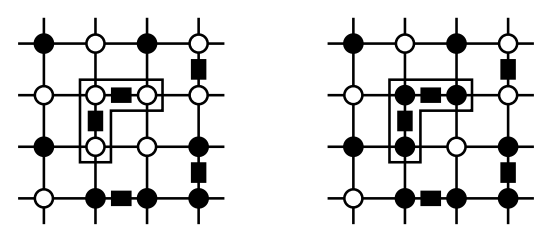
\includegraphics[width=0.7\linewidth]{clusters_sw_theory.png}
    \caption{A spin configuration (circles) in which filled bonds (thick lines between circles) have
been cast between equal spins according to the appropriate probability}
    \label{fig:enter-label}
\end{figure}

For a given spin configuration, we define the probability of a bond configuration corresponding to the weight in equation \ref{eq:weight}:
\begin{equation}
    P = \frac{F(i,j)}{F(0) + F(1)}, 
\end{equation}
Hence, the probability of the filled bond is:
\begin{equation}
    P = 1 - \mathrm{e}^{-2J/T} , \hspace{0.3cm} \text{if} \hspace{0.3cm} \sigma_{i(b)} = \sigma_{j(b)}
\end{equation}
\begin{equation}
    P = 0 , \hspace{0.3cm} \text{if} \hspace{0.3cm} \sigma_{i(b)} \neq \sigma_{j(b)}
\end{equation}

\vspace{0.3cm}
Now, based on the above mathematical formulation, we can present how to run up the SW algorithm, starting from the initial configuration of our random choice ($P(C_0)$): 
\begin{enumerate}
    \item Specifying the coordinates to each lattice sites and then one form a bond between every pairs of nearest neighbours, with a probability $p_{ij} = 1 - \mathrm{e}^{-2 \beta J}$.
    
    \item All spins that are connected, directly or indirectly, via bonds belong to a single cluster. Thus, the bond assignment procedure divides the system into clusters of parallel spins (a so called cluster decomposition). The bond probability (and hence the typical cluster size) grows with increasing coupling strength $\beta J$ (decreasing temperature). For a finite temperature, $p_{ij} < 1$, and hence a cluster is generally a subset of all spins of a given sign. In common words, two spins of the same sign need not belong to the same cluster, even if these spins are adjacent on the lattice.
    
    \item All spins in each cluster are flipped collectively with a probability $\frac{1}{2}$. The reason for choosing half is one's symmetric choice than any physical intuition. Of-course one can choose any number between 0 to 1, and the algorithm works well, provided we do not biased the aspect by choosing specifically 1 or 0. 
    
    \item All bonds are erased and the “cluster move” is complete; a new spin configuration has been created, and then one procceds to step -1 again. 
    
\end{enumerate}
The clusters created in the Swendsen–Wang algorithm have a structure that is very efficient at destroying non-local correlations (\textit{as all the spins are correlated to each other, because when one measure energy of one spins, it requires information about the other nearest 4, and this chain continues upto the length of the lattice, and this correlation is destroyed here}). As a result, the dynamical critical exponent z is lowered to a much smaller value and independent configurations can be generated at a much faster rate than with a single-spin flip algorithm. This advantage only holds in the vicinity of the critical temperature,
which also happens to be the most interesting point in the study of lattice spin models such as the Ising model. \\

This method ofcourse satisfy the detailed balance condition\supercite{SW} and also the dynamic
critical exponent z for the SW method is much smaller, $z = 0.35$ and our calculated value is 0.377. \\

\vspace{0.2cm}
\noindent {\large \textbf{Wolff Algorithm}} \\

Wolff\supercite{Wolff_algo} introduced a so-called single-cluster variant of this algorithm. In
the SW algorithm, small and large clusters are created. While the destruction of critical correlations is predominantly due to the large clusters, a considerable amount of effort is spent on constructing the smaller clusters. In Wolff’s implementation, no decomposition of the entire spin configuration into clusters takes place. Instead, only a single cluster is formed, which is then always flipped. If this cluster turns out to be large, correlations are destroyed as effectively
as by means of the large clusters in the SW algorithm, without the effort of creating the smaller clusters that fill up the remainder of the system. If the Wolff cluster turns out to be small, then not much is gained, but also not much computational effort is required. As a result, critical slowing down is suppressed even more strongly than in the SW algorithm, and the dynamical critical exponent z is even smaller.

\begin{enumerate}
    \item A spin $i$ is selected at random.
    \item All nearest neighbors $j$ of this spin are added to the cluster with a probability $p_{ij} = 1 - \exp(-2\beta J)$, provided spins $i$ and $j$ are parallel and the bond between $i$ and $j$ has not been considered before.
    \item Each spin $j$ that is indeed added to the cluster is also placed on the stack. Once all neighbors of $i$ have been considered for inclusion in the cluster, a spin is retrieved from the stack and all its neighbors are considered in turn for inclusion in the cluster as well, following step (2).
    \item Steps (2) and (3) are repeated iteratively until the stack is empty.
    \item Once the cluster has been completed, all spins that belong to the cluster are flipped with $\frac{1}{2}$ probability.
\end{enumerate}

This method ofcourse satisfy the detailed balance condition\supercite{Wolff_algo} and also the dynamic
critical exponent z for the Wolff is even much smaller than the previous 2 methods $z = 0.20$ and our calculated value shows promising result of 0.19. \\

\subsection{Cluster algorithms for off-lattice model}
After the success of SW and Wolff algorithm, these models found huge applications in off-lattice model. The geometric cluster algorithm described is formulated for particles that interact via hard-core repulsion's only. We have discussed the case of that hard core repulsion's only between the spheres. 
\begin{equation}
    V(r_{1}, r_{2}) = \begin{cases}
0 & \text{if } |r_{1} - r_{2}| > \sigma, \\
\infty & \text{if } |r_{1} - r_{2}| < \sigma.
\end{cases}
\end{equation}
To devise a general cluster flipping method for off-lattice systems, e.g. fluids, was not immediately obvious. The first step was taken by Dress and Krauth in 1995 who used geometric operations to design a cluster algorithm for hard spheres. 
\begin{enumerate}
    \item In a given configuration C, a \enquote{pivot} is chosen at random.
    \item A particle i at position $r_i$ is selected as the first particle that belongs to the cluster. This particle is moved via a point reflection with respect to the pivot. In its new position, the particle is referred to as $i'$, at position $r_i'$
  \item Each particle j that interacts with $i$ or $i'$ is now considered for addition to the cluster. A particle j that interacts with i both in its old and in its new position is nevertheless treated once. Unlike the first particle, particle j is point-reflected with respect to the pivot only with a probability $p_{ij} = \max[1 - \exp(-\beta \Delta_{ij}), 0]$, where $\Delta_{ij} = V(|\mathbf{r}_i' - \mathbf{r}_j|) - V(|\mathbf{r}_i' - \mathbf{r}_j|)$.
    \item Each particle $j$ that is indeed added to the cluster (i.e., moved) is also placed on the stack. Once all particles interacting with $i$ or $i'$ have been considered, a particle is retrieved from the stack and all its neighbors that are not yet part of the cluster are considered in turn for inclusion in the cluster as well, following step 3.
    \item Steps 3 and 4 are repeated iterative until the stack is empty. The cluster move is now complete.
\end{enumerate}

The very good description of the GCA (Geometric cluster analysis) is given in these lecture notes.\supercite{wow}
\subsection{Bootstrapping}
The ensemble averages of the thermodynamic quantities listed in section 5 are determined by the bootstrapping technique. For a given data set $d_{MC}$ of the MC simulations consisting of $K$ data points, the bootstrapping technique randomly picks K data points from this set. From these randomly picked $K$ data points the quantity $Q$ is calculated in the same manner as it would have been calculated from the original data set. This process is repeated many times (say $M$) times for the same data set $d_{MC}$. The $M$ different values of Q are then used to determine the average and the standard deviation of Q.

\subsection{Trial function for obtaining the exponents}
The critical exponents corresponding to the quantities mentioned in table 1 are determined by fitting a trial function to the simulated data for $C_v, \chi, m$. The trail function for m and $\chi$ is given by:
\begin{equation}
    f_{trial} = a|\Tilde{T}|^b  \label{eq:trial_critical}
\end{equation}
where, $\Tilde{T} = T - T_c$ and a, b are the fitting parameters. In the case of magnitization, the absolute sign of temperature is just replaced by $\Tilde{T}$. \\

The dynamic critical exponent z can be extracted from the peak position of a quantity. In general the peak position scales as $T_{peak} \propto L^z$. Hence, data for multiple system sizes is needed. This simulated data is fitted to the following trial function:
\begin{equation}
    f_{trial, z} = L^{-a} + c,  \label{eq:trial_dynamical}
\end{equation}
where $L$ is the length of the lattice and a, c are the fitting parameters. We will choose the magnetic susceptibility chosen to determine z since its data shows clearly defined peaks unlike specific heat.


\section{Thermodynamics quantities}
In the simulation, we have computed the following thermodynamic quantities from there standard formula. 
\begin{equation}
     m = \frac{1}{N} \langle sum_{i} \sigma_{i} \rangle
\end{equation}
Magnetization, this is the ordered parameter for the ferromagnetic phase transition. This becomes zero after the critical temperature, and was aliged in the same direction below critical temperature. \\

\noindent The fluctuations of the energy of the system are used to calculate the specific heat of the system.
\begin{equation}
    C_v = \frac{k_{B} \beta^2}{N} (\langle  E^2 \rangle - (\langle E \rangle)^2 )
\end{equation}
The magnetic susceptibility ($\chi$) is a measure of magnetic properties of a material. It indicates whether a material is attracted to or repelled by a magnetic field.

\begin{equation}
    \chi = \beta N (\langle  m^2 \rangle - (\langle m \rangle)^2 )
\end{equation}
Since the magnetic susceptibility over temperature is a measure of the change of magnetisation over temperature, a sharp peak is expected at the critical temperature due to the sudden change of the magnetisation at the phase transition.

\section{Results}
The results presented in this section are for a 2D Ising lattice of sides $L = 40$ unless specifically stated otherwise. The temperature interval chosen starts from 1.5 going up to 1.5 in 80 equidistant steps. Simulations start with all spins in the up position. At every temperature the simulation runs for 5100 MC steps of which the last 5000 MC steps are used to determine the quantities. The first 100 MC steps are needed for the system to adapt to the new temperature (this is called as thermalization). Furthermore, uncertainties are calculated using the bootstrap method with $M$ = 1000.

\subsection{Thermodynamic quantities against temperature}

The graph for the various thermodynamic quantities using SW algorithm are presented here. The similar graphs are also generated for Wolff as well as Metropolis algorithm, just the difference is which algorithm takes what amount of time, and how far in time correlation dies.  The graphs for magnetization, specific heat per spin and magnetic susceptibility per spin is presented in figure \ref{fig:mani}, \ref{fig:cv} and \ref{fig:magnetic sus} respectively. \\

As expected the peak in the spectrum becomes less flattened when the system size increases and will eventually reach the relation stated in table 1 near the critical temperature. It can also be seen that the location of the peak shifts to lower temperatures when L increases and will eventually go asymptotically to the theoretical value 2.269 for $L \rightarrow \infty$. Similarly for the magnetic susceptibility, the peak within the spectrum becomes more
apparent for larger system sizes and also shifts to lower temperatures, and in the theoretical limit of $L \rightarrow \infty$ the peak will be located at the critical temperature. This is as expected since it should behave as the variance of the magnetisation. \\

\begin{figure}[htbp]
    \centering
    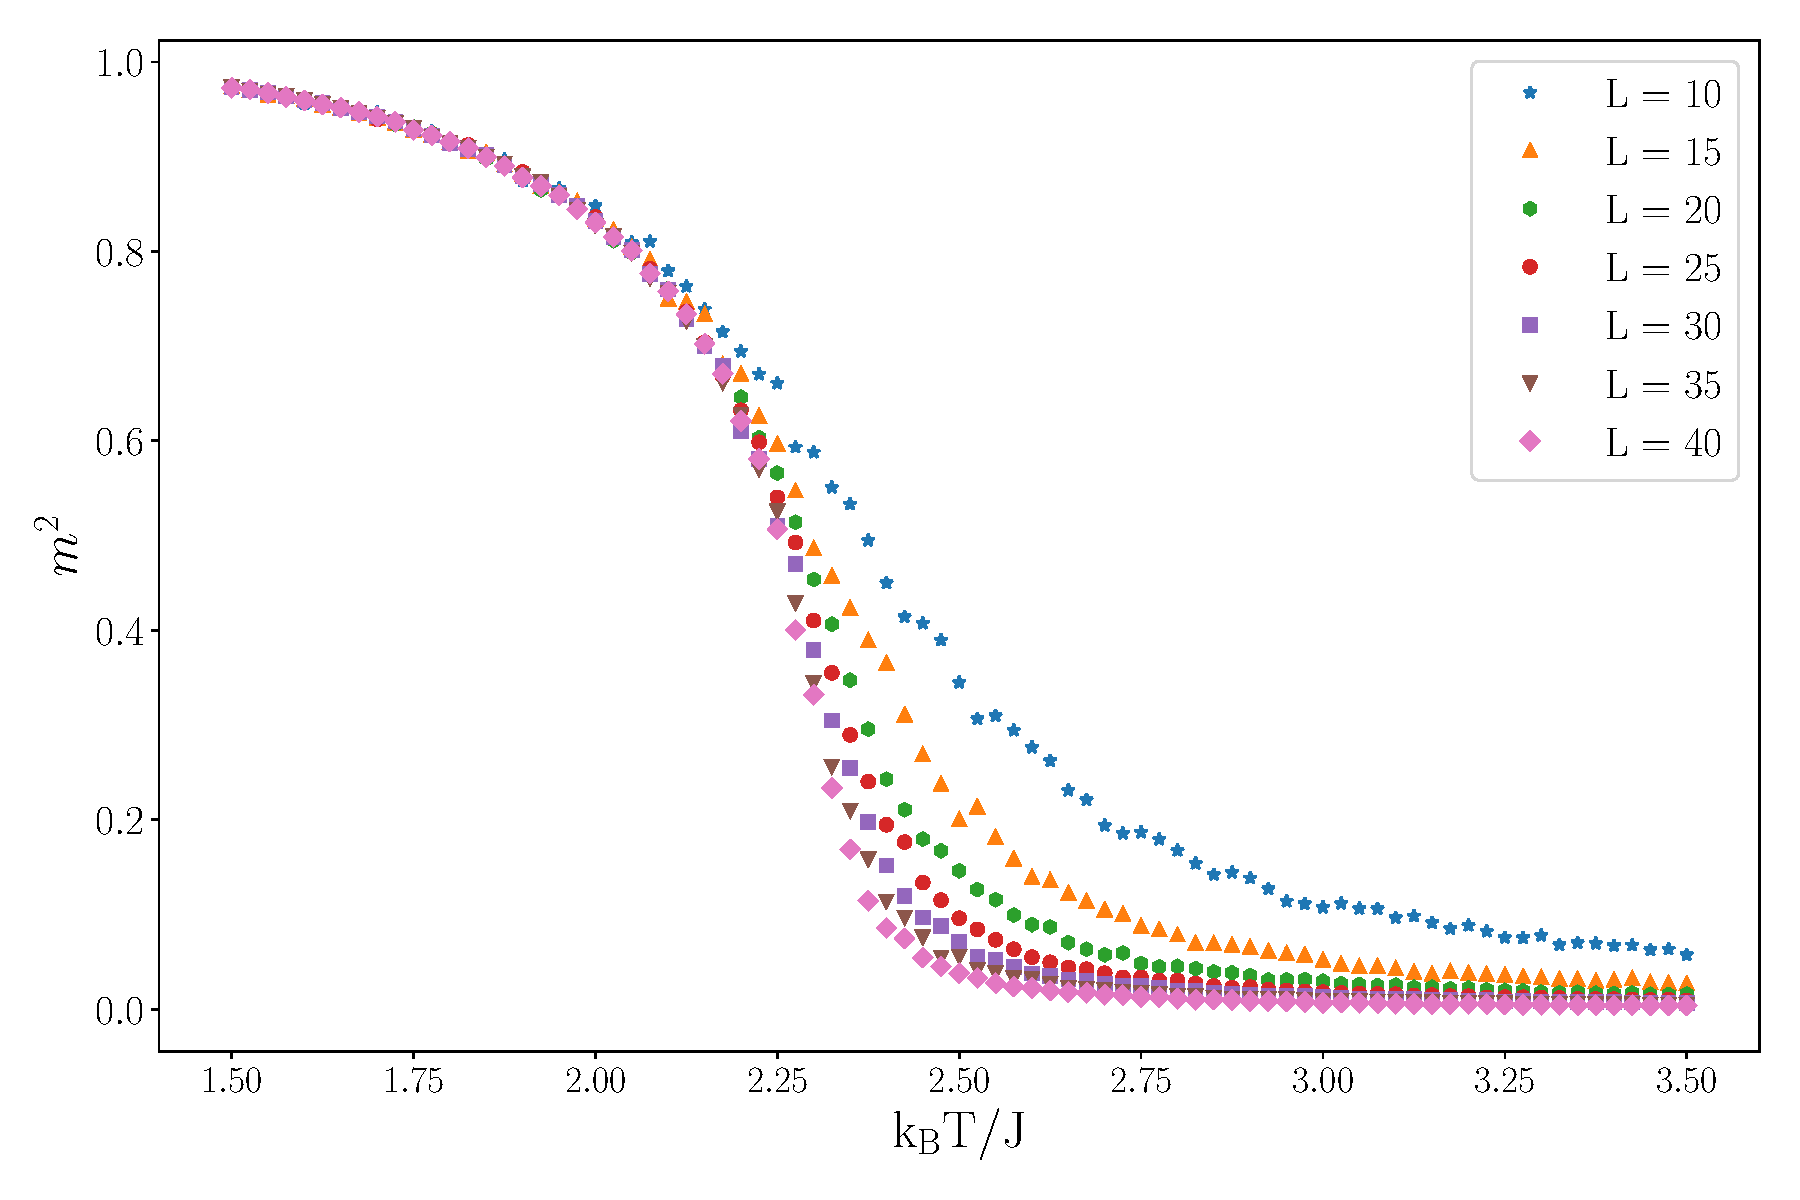
\includegraphics[scale = 0.4]{triple_2000_magnetisation.pdf}
    \caption{Graph showing the magnetization (actually it's square for symmetry reason) per spin against temperature using SW algorithm for different lattice sizes.}
    \label{fig:mani}
\end{figure}

\begin{figure}[htbp]
    \centering
    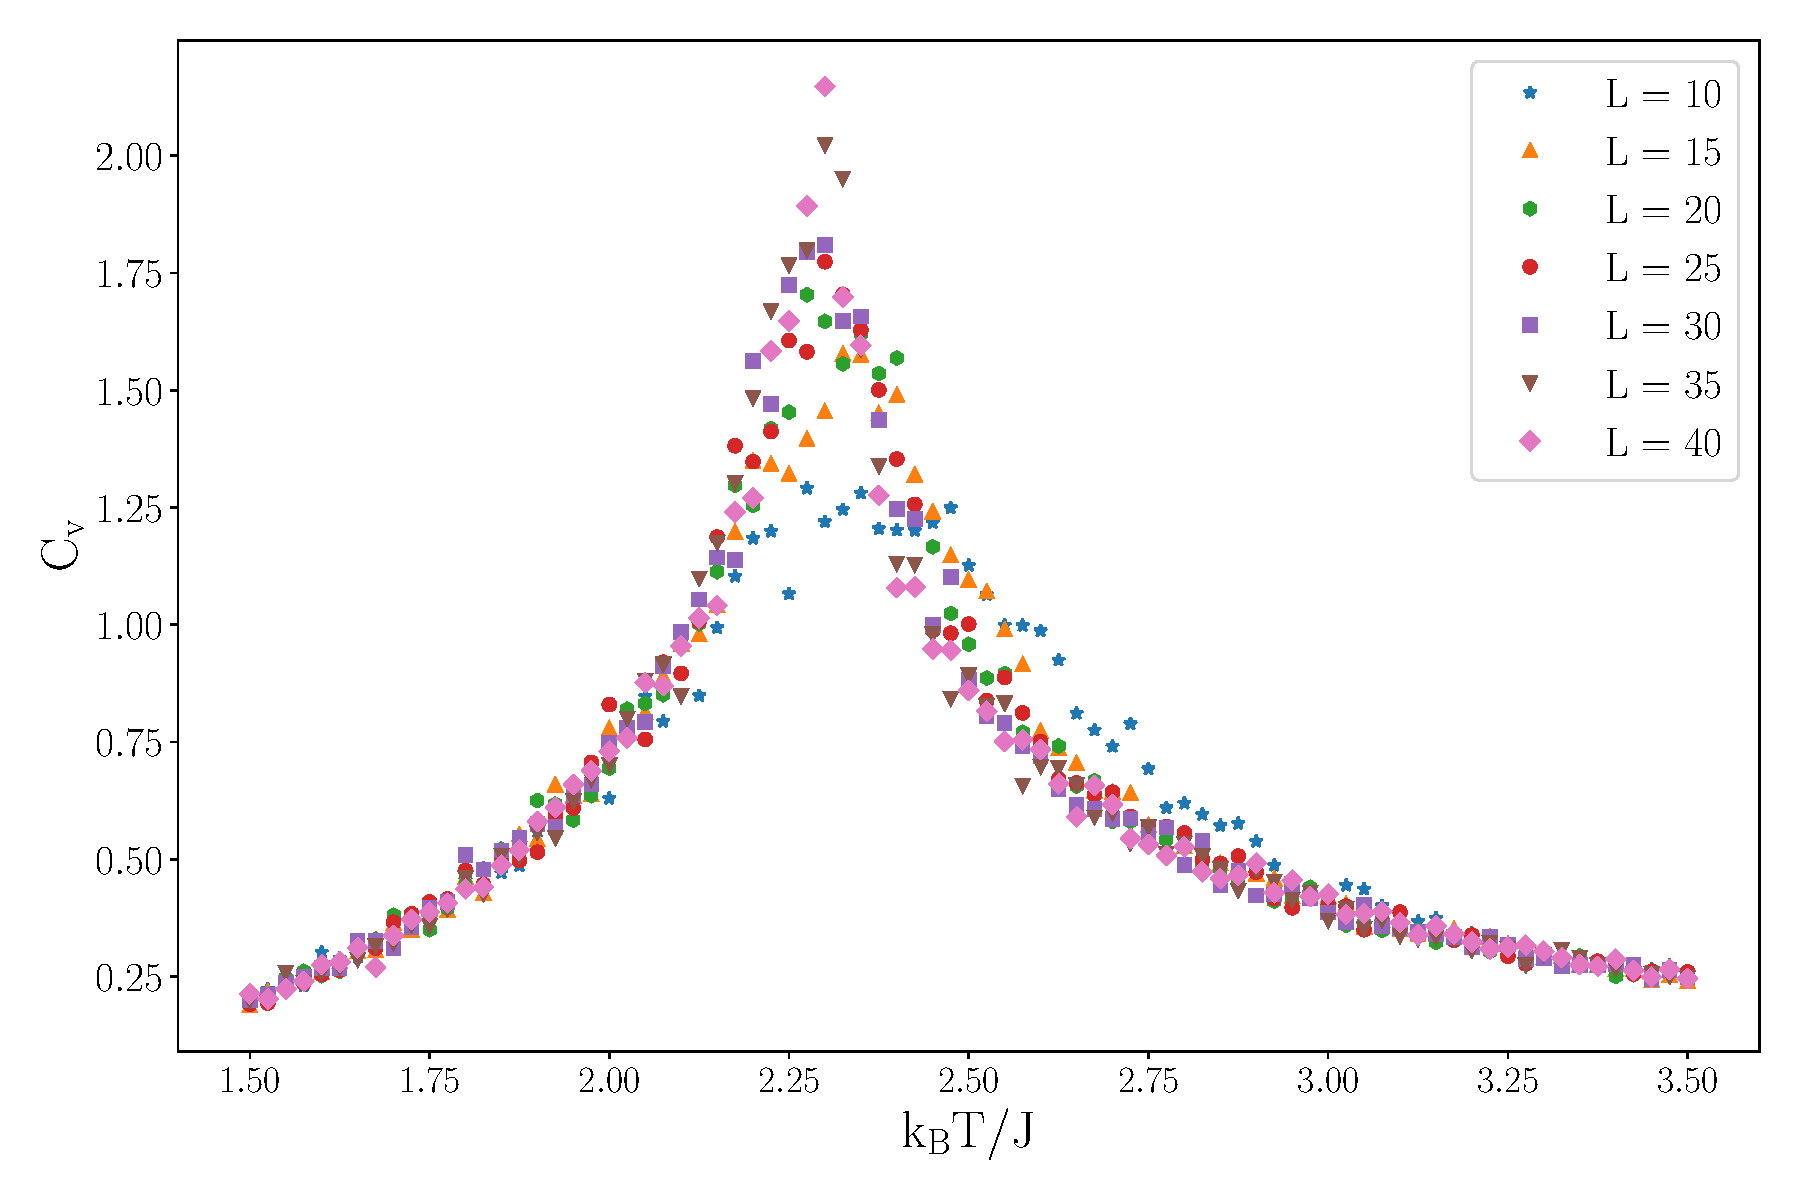
\includegraphics[scale = 0.4]{triple_2000_c_v.pdf}
    \caption{Graph showing the specific heat per spin against temperature using SW algorithm for different lattice sizes.}
    \label{fig:cv}
\end{figure}

\begin{figure}[htbp]
    \centering
    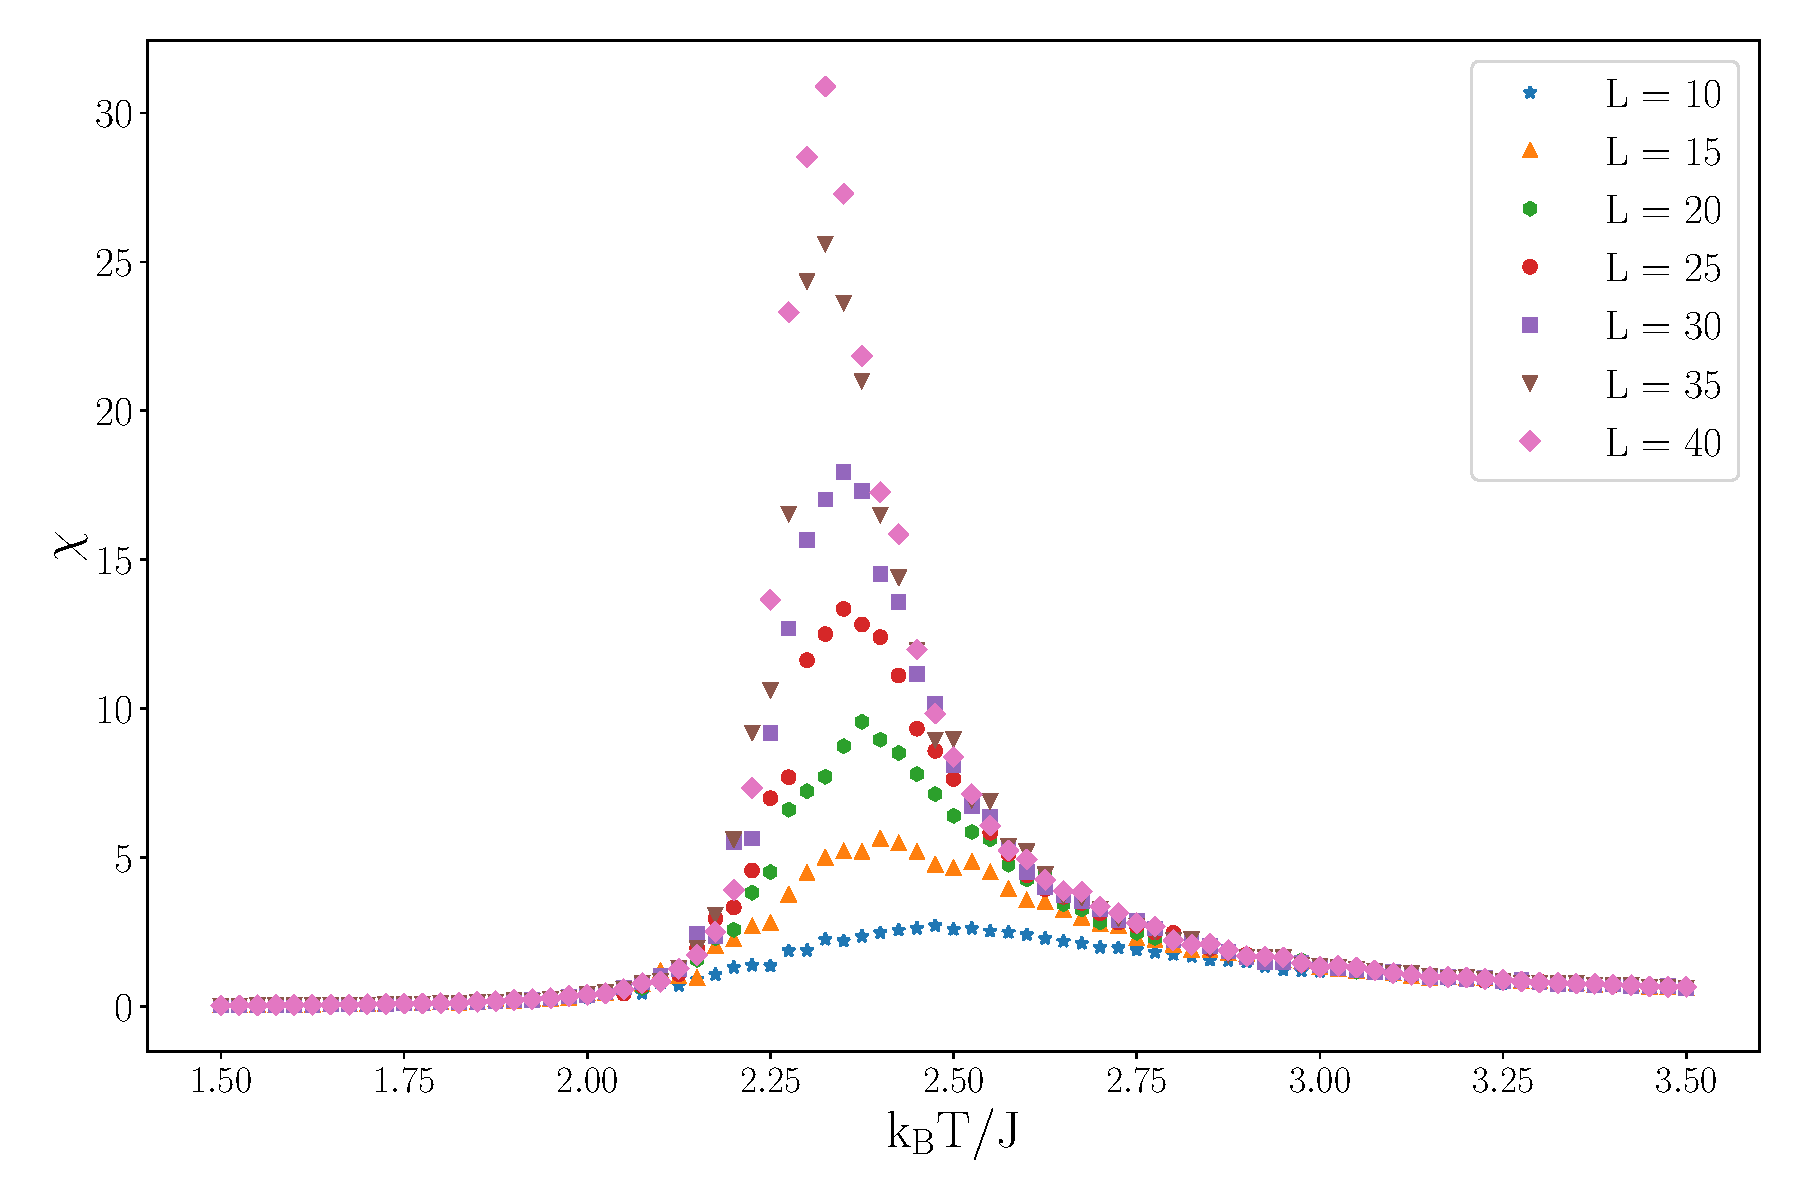
\includegraphics[scale = 0.4]{triple_2000_chi.pdf}
    \caption{Graph showing the magnetic susceptibility against temperature using SW algorithm for different lattice sizes.}
    \label{fig:magnetic sus}
\end{figure}


The critical temperature is determined from the $\chi$ peak at L = 40, because this has a more distinctive peak than the specific heat. From figure \ref{fig:magnetic sus}, the highest peak is found to be at T = 2.30

\subsection{Exponents}
Already presented theoretically, these exponents are then calculated through simulations. We calculated both the dynamic as well as critical exponents for all the three algorithms.

\subsubsection{Dynamical exponent}
To acquire data for multiple system sizes, $L$ is varied from 10 to 40 in steps of 5. This is done for
2100 MC steps in stead of 5100 to save on computation time. Fitting to equation \ref{eq:trial_dynamical} results for the SW algorithm in $z_{\chi}$ = 0.377 and for Wolff  $z_{\chi}$ = 0.19, which agrees from there papers.\supercite{Wolff_algo}\supercite{SW} We tried to compute  $z_{\chi}$ for metropolis as well, but the errors are as big as the quantity itself, so nothing can be predicted. This problem might be overcome if we increase the length of the lattice but this is not feasible option is quite a less time.

The graph for the auto-correlation time against lattice size is shown, from where we extracted z for SW. 
\begin{figure}[htbp]
    \centering
    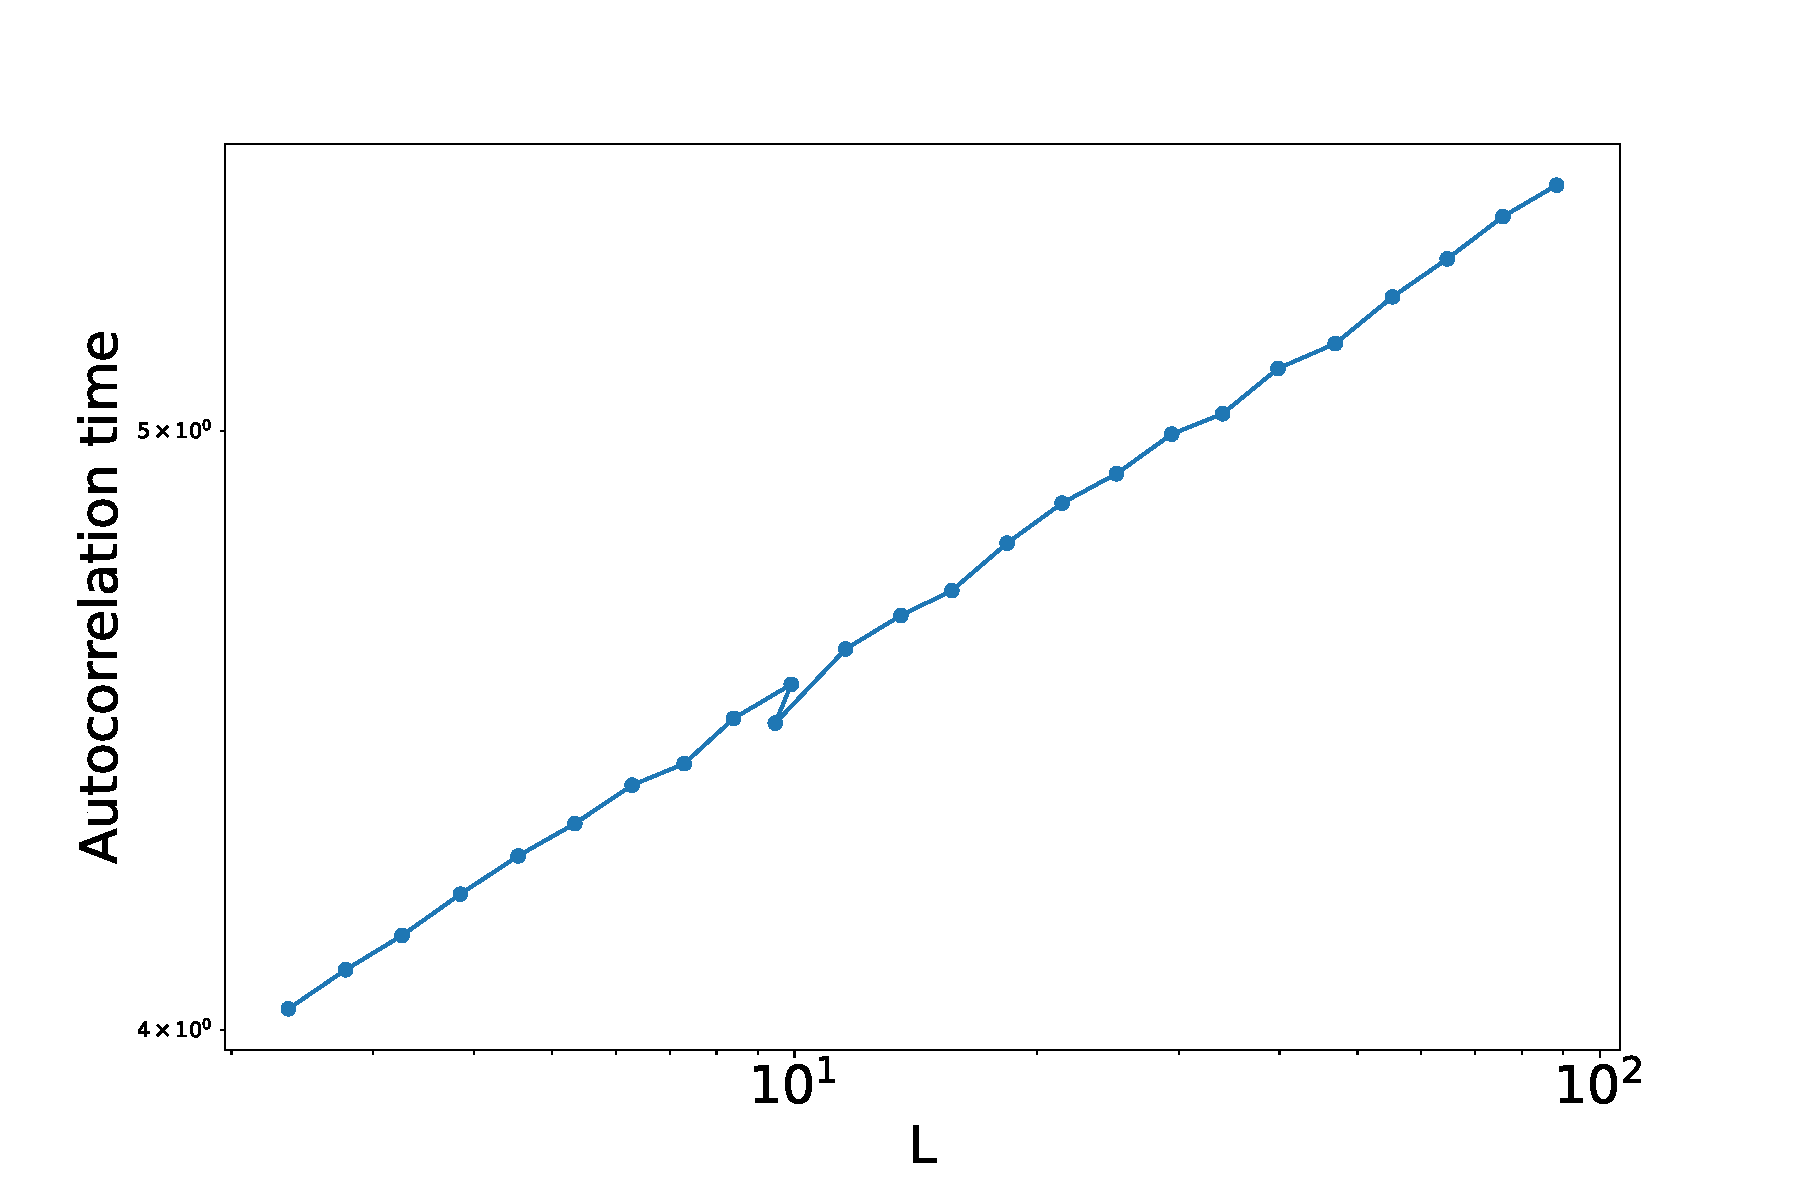
\includegraphics[scale = 0.4]{autocorrelation.pdf}
    \caption{Graph showing the autocorrelation time against lattice size for SW algorithm. Form here, value of z was found to be 0.37 against the SW value 0.35\supercite{SW}}
    \label{fig:magnetic sus}
\end{figure}

\begin{figure}[htbp]
    \centering
    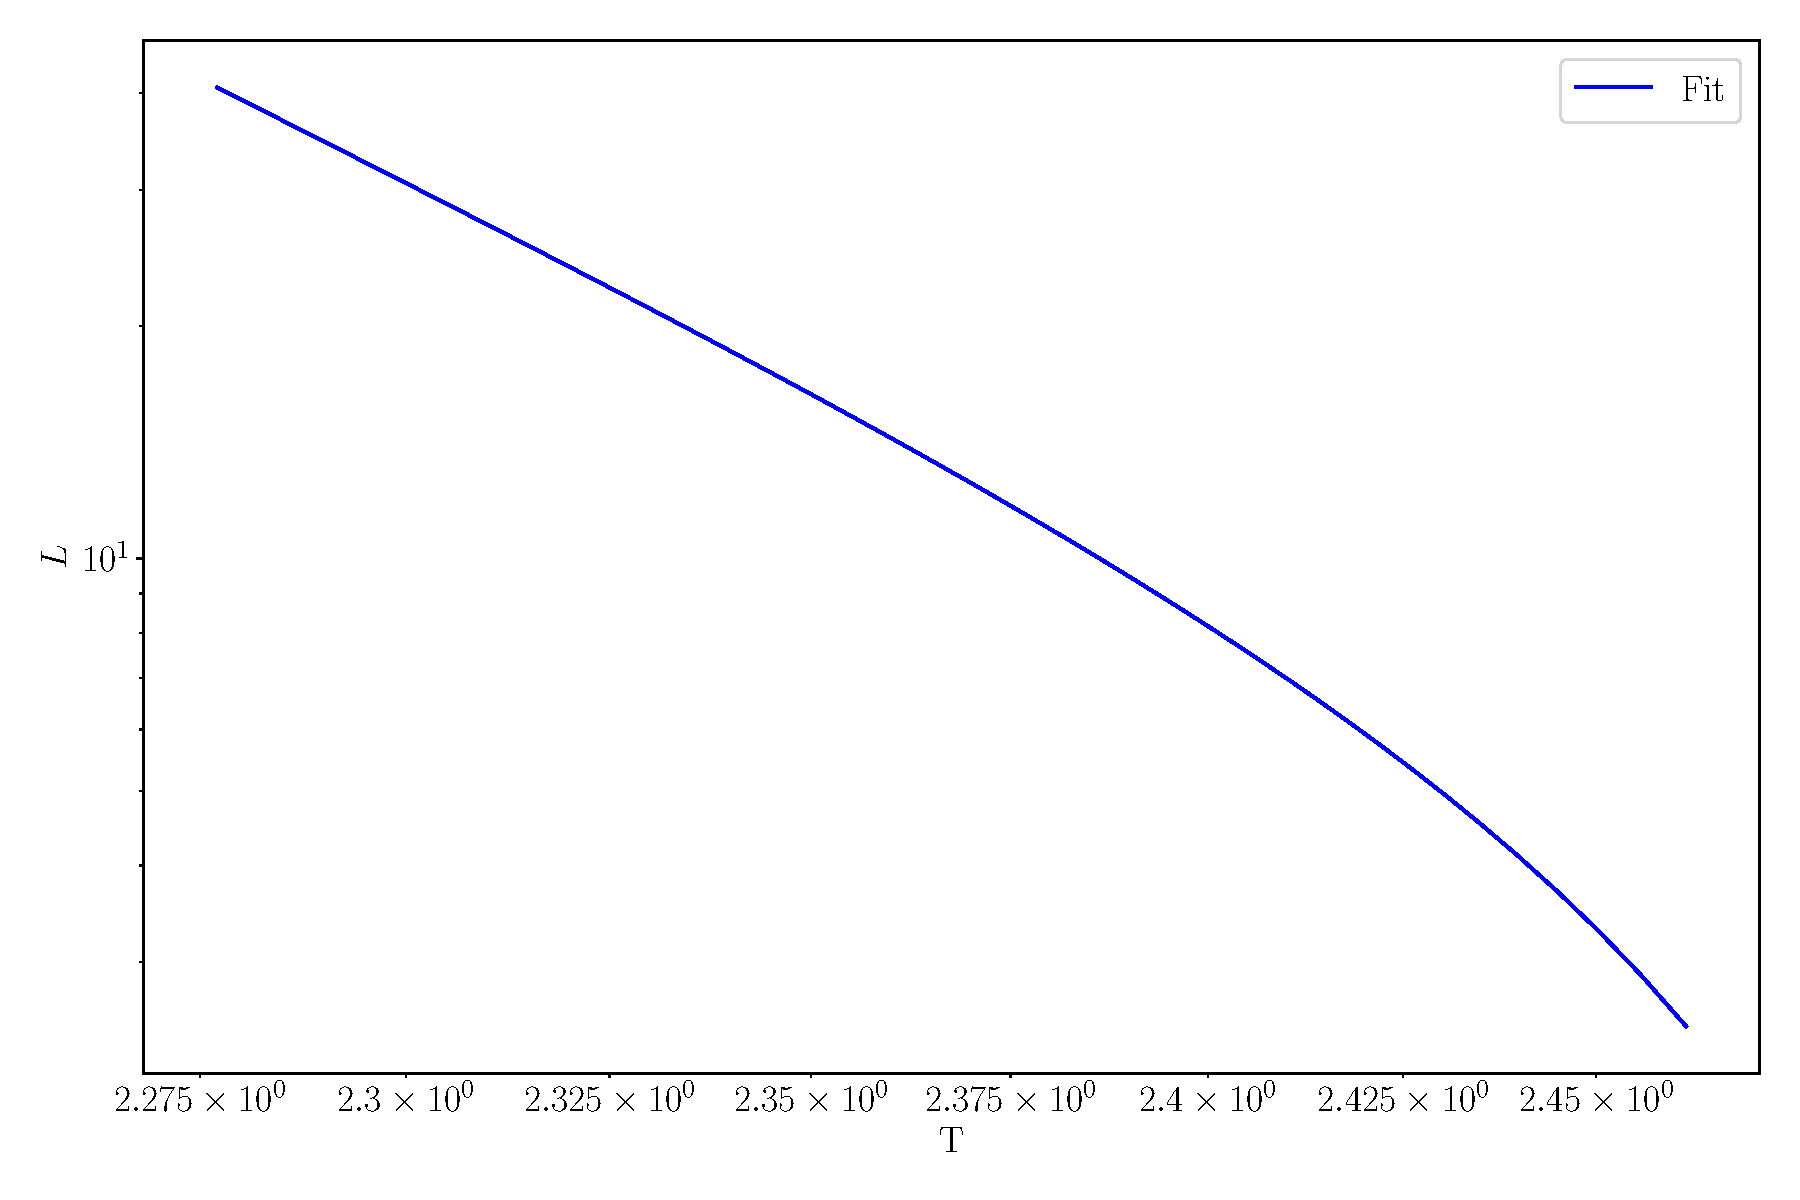
\includegraphics[scale = 0.35]{triple_fit_chi.pdf}
    \caption{Graph showing the lattice size against critical temperature for wolff algorithm. Form here, value of z was found to be 0.19 against the value 0.20 obtained by Wolff\supercite{Wolff_algo}}
    \label{fig:magnetic sus}
\end{figure}

\subsubsection{Critical exponents}
The critical exponents for the magnetisation and the magnetic susceptibility are determined by
fitting the trial function in equation \ref{eq:trial_critical} to the acquired data. The trial
function is defined with respect to $T - T_c$ while the simulated data is defined with respect to $T$, so we translated all the $T$'s to, $T - T_c$, which results in an axis with both $T - T_c > 0$ and  $T - T_c < 0$. The fit to te magnetic susceptibility is shown in figure \ref{fig:log_mag_spe}

\begin{figure}[htbp]
    \centering
    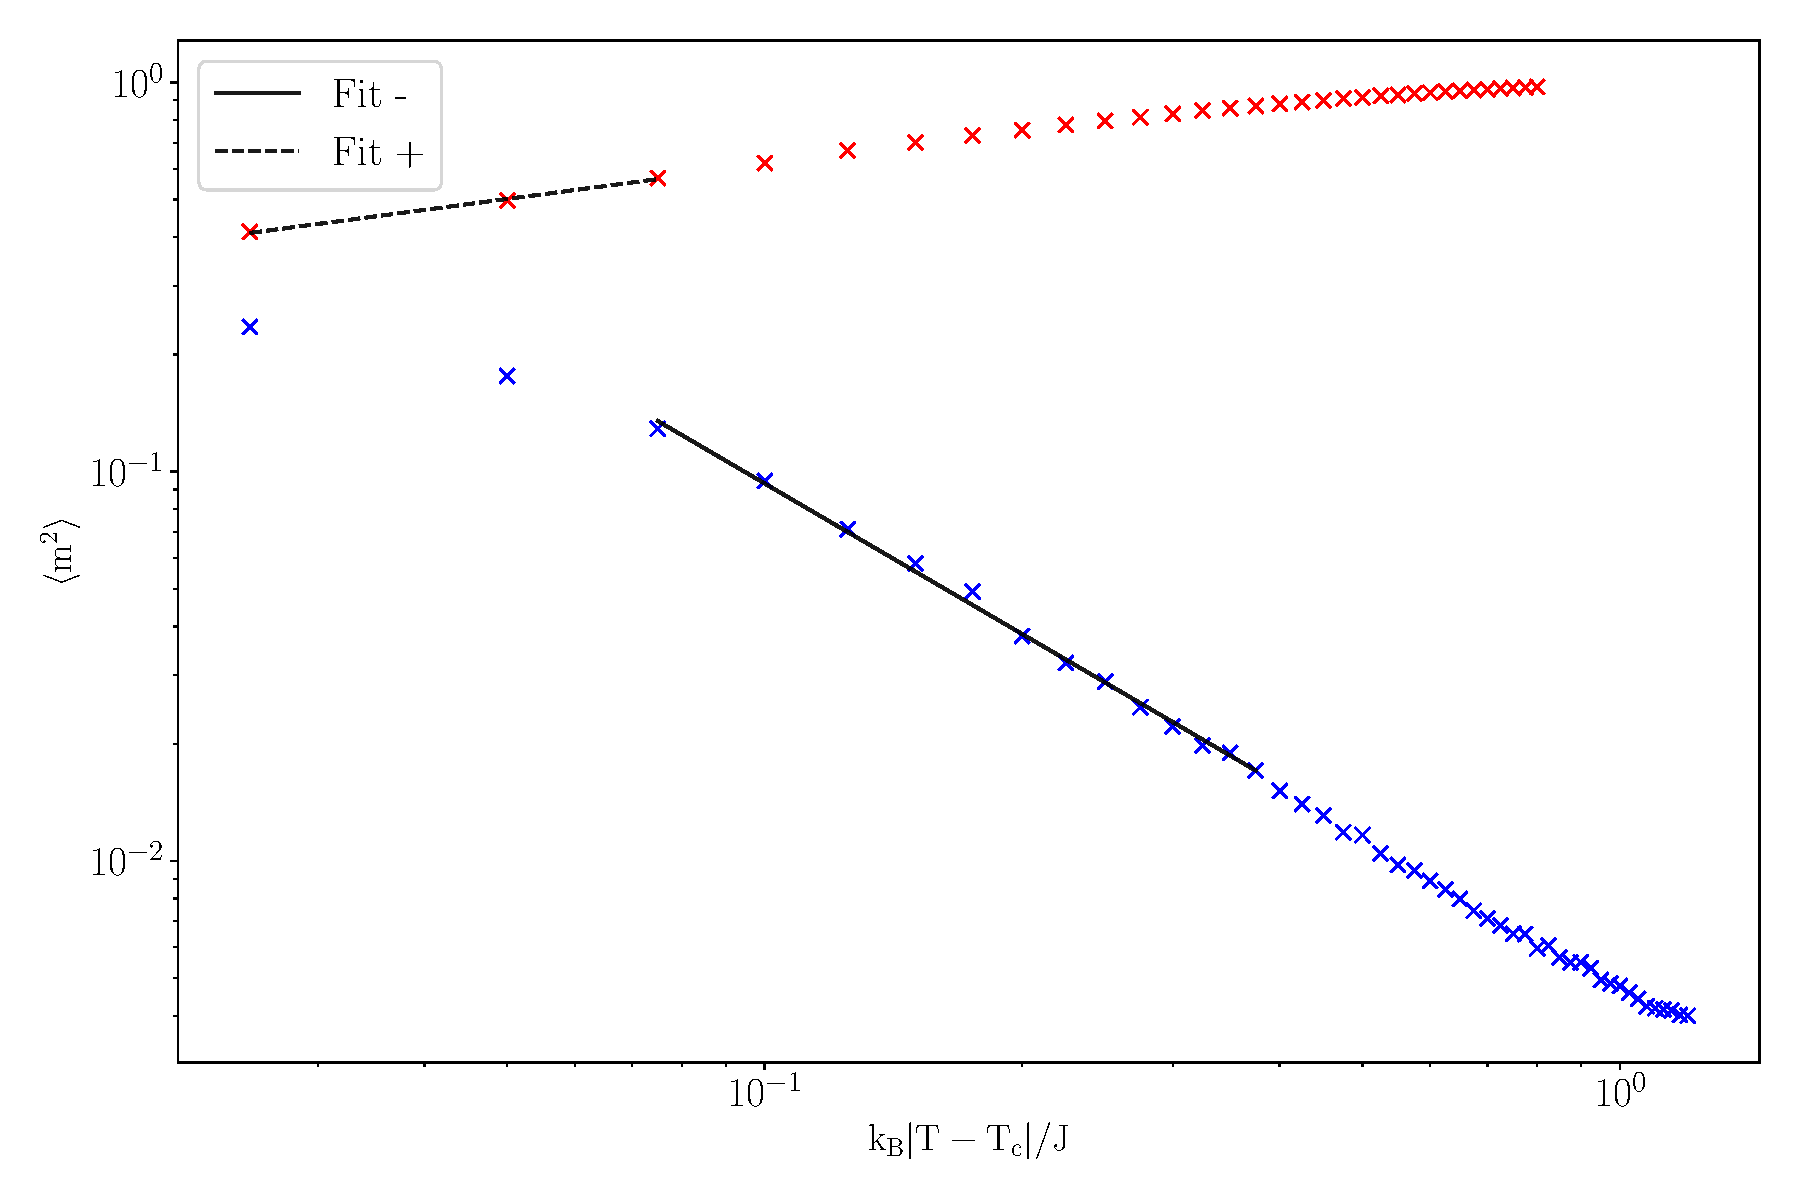
\includegraphics[scale = 0.3]{L40_SW_5000_magnetisation_fitted_log.pdf}
    \caption{Logarithmic plot of $\langle m^2 \rangle$ including fit. For $T - T_c > 0$ is in blue with accompanying fit ‘Fit +’ and for $T - T_c < 0$ in red with ‘Fit -’.}
    \label{fig:log_mag_spe}
\end{figure}

\begin{figure}[htbp]
    \centering
    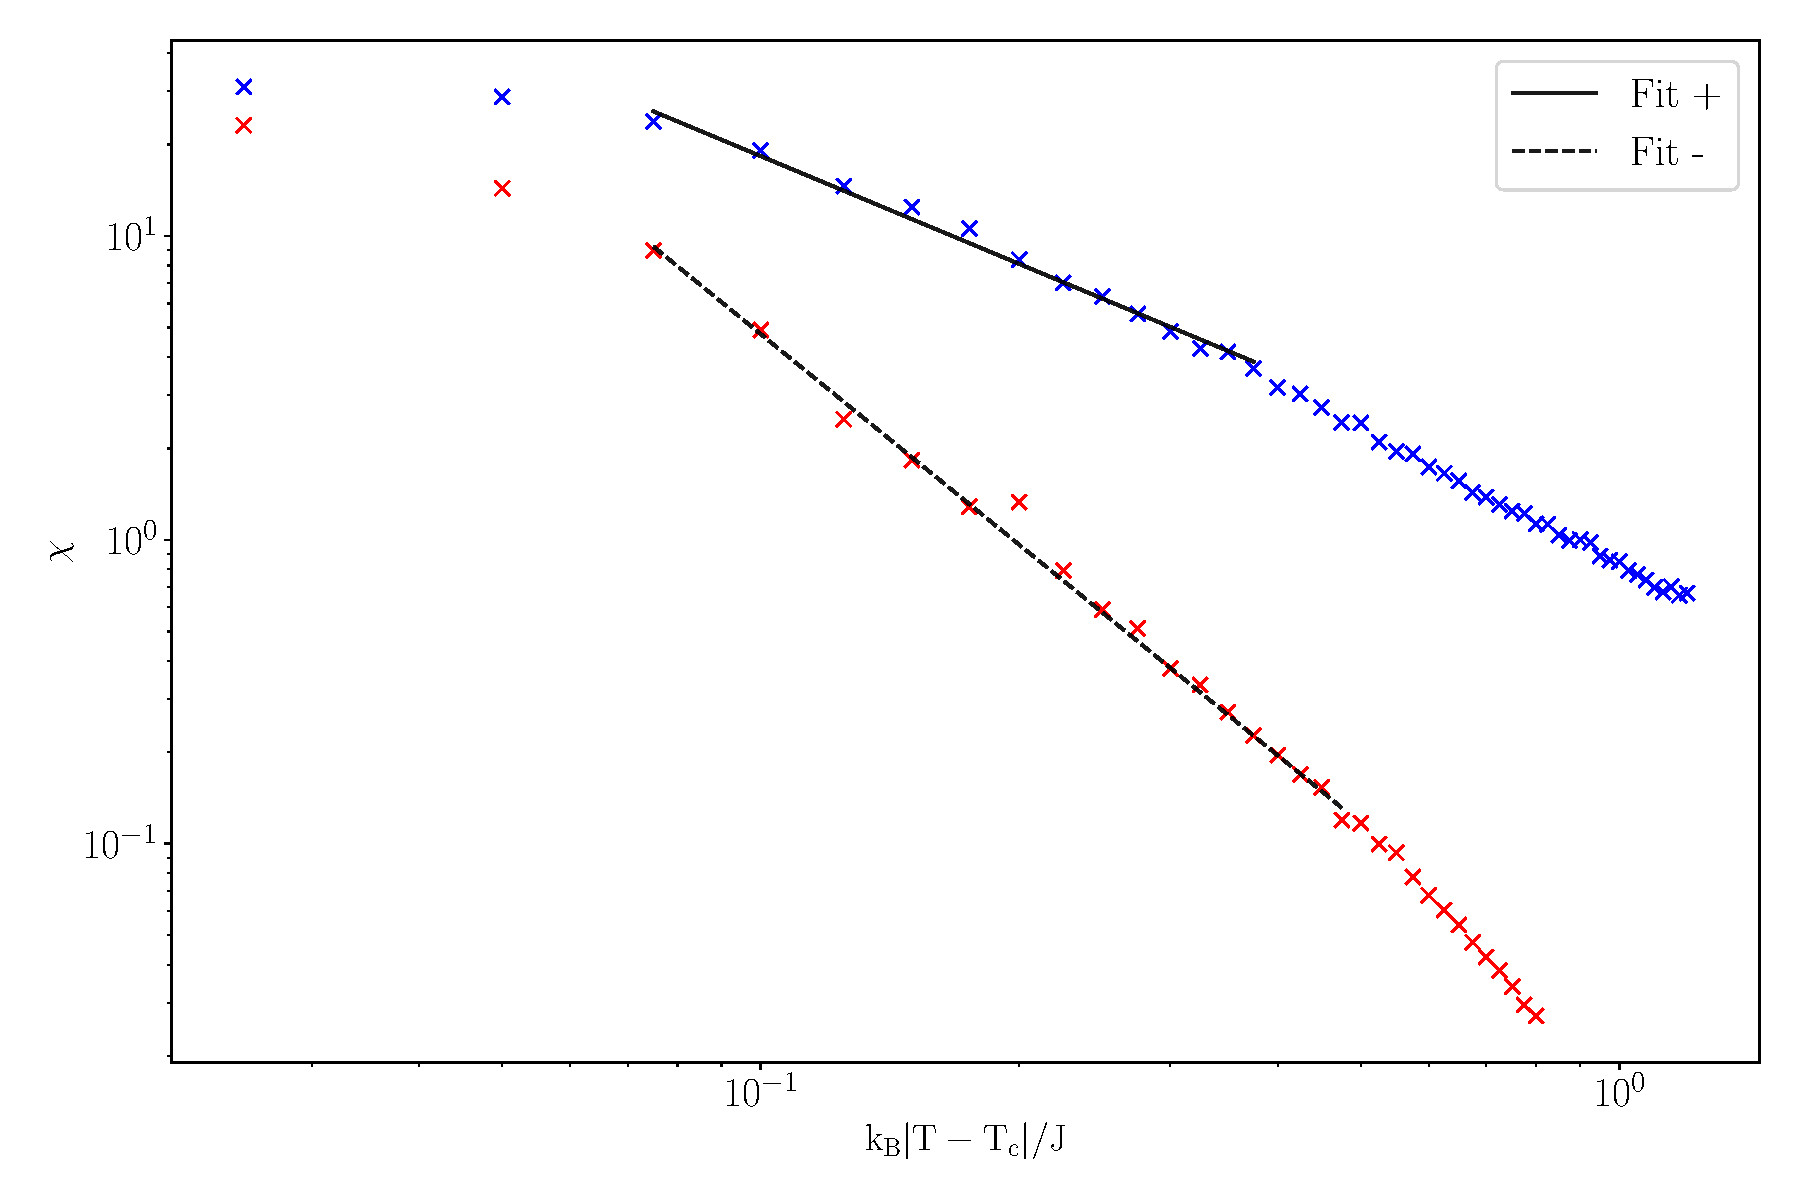
\includegraphics[scale = 0.3]{L40_SW_5000_chi_fitted_log.pdf}
    \caption{Logarithmic plot of $\chi$ including fit. For $T - T_c > 0$ is in blue with accompanying fit ‘Fit +’ and for $T - T_c < 0$ in red with ‘Fit -’.}
    \label{fig:log_mag_sus}
\end{figure}
From figure \ref{fig:log_mag_sus}, one can note that the flattening of the curve for $T - T_c$ close to 0, and also different slopes of the curve for $T - T_c < 0$ and $T - T_c < 0$. The reason for such is just the finite dimensions of the system. The corresponding critical exponents obtained from wolff and SW are also shown in the table \ref{tab:sw_critical} and \ref{tab:wolff_critical}.

\begin{figure}[htbp]
    \centering
    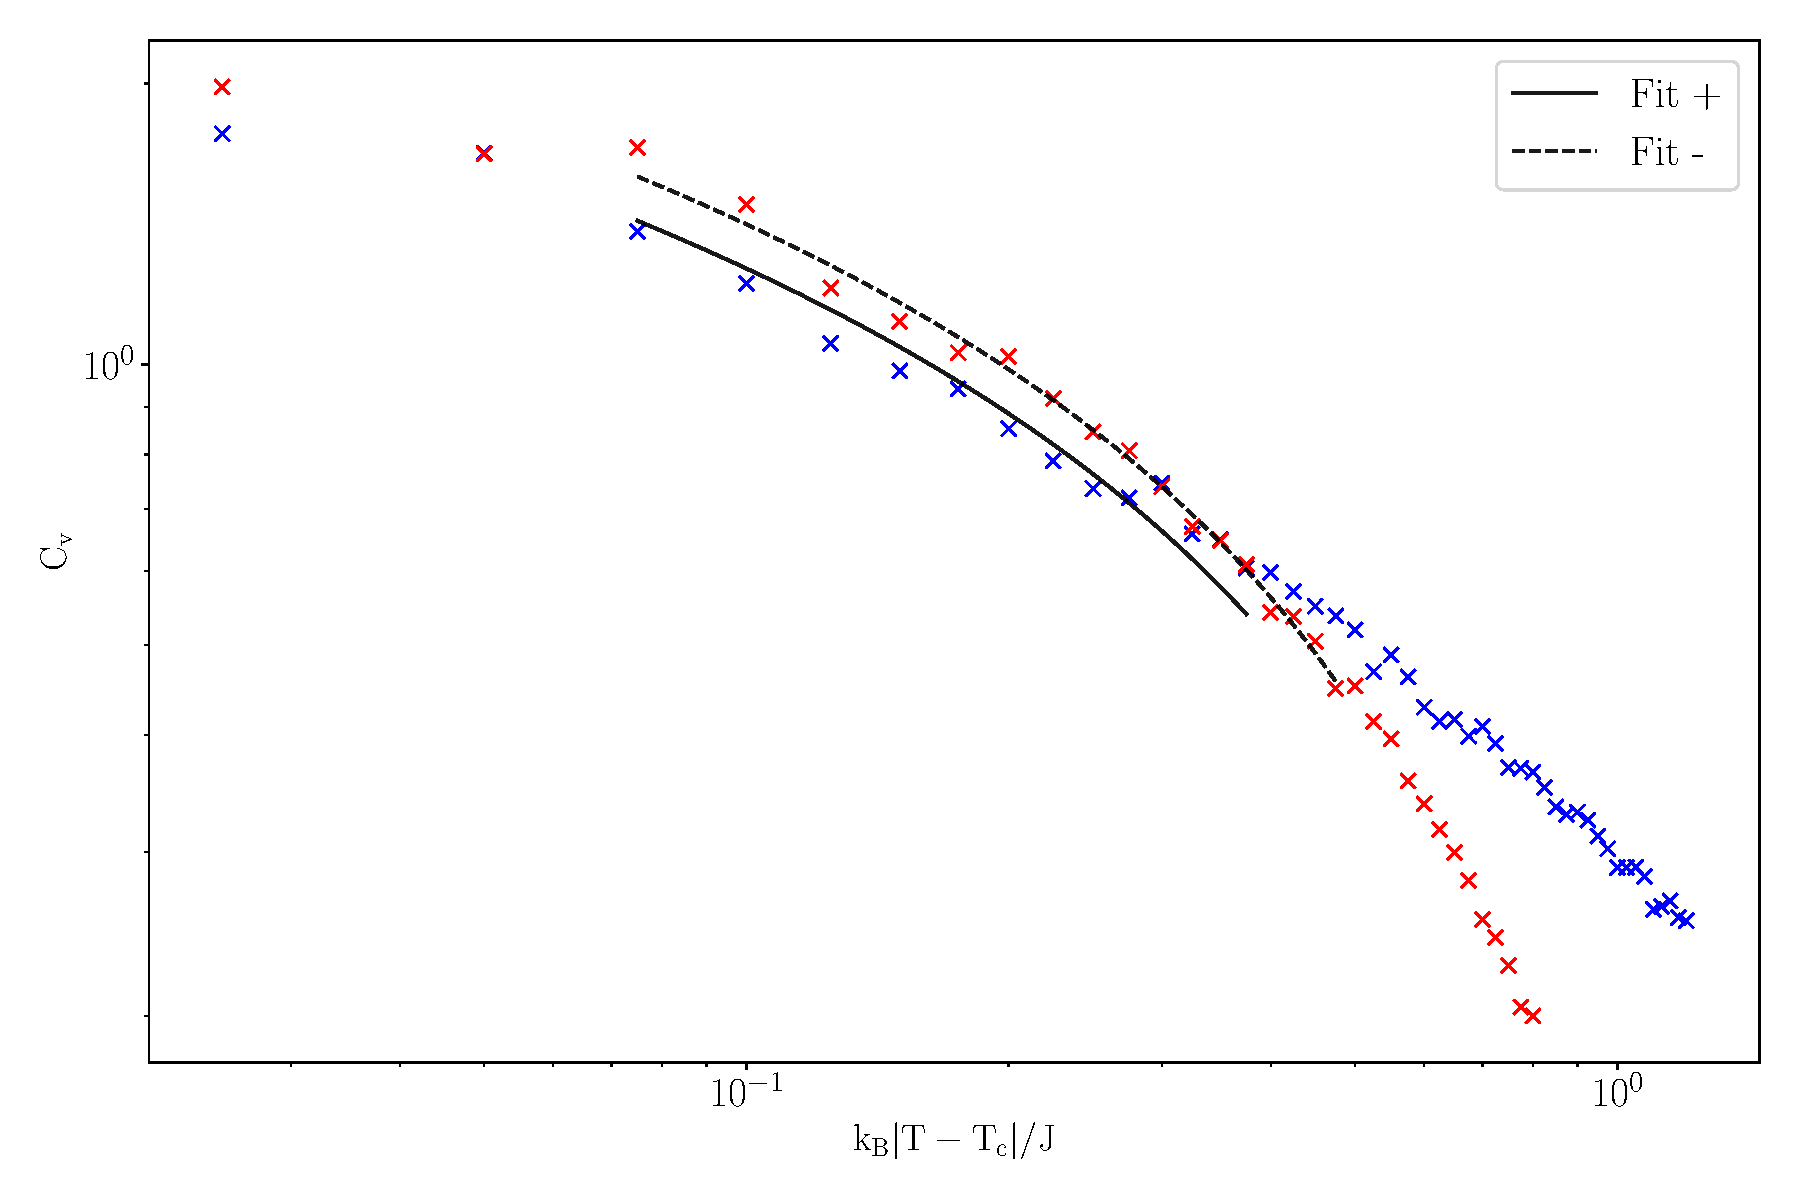
\includegraphics[scale = 0.35]{L40_SW_5000_c_v_fitted_log.pdf}
    \caption{Logarithmic plot of $c_v$ including fit. For $T - T_c > 0$ is in blue with accompanying fit ‘Fit +’ and for $T - T_c < 0$ in red with ‘Fit -’.}
    \label{fig:log_cv_spe}
\end{figure}

One can now note from table \ref{tab:sw_critical}, exponents corresponding to $\langle m \rangle$, i.e., $\beta$ shows very accurate answer as comparison to theoretical value in table 1. But, this is not the perfect case with $\gamma$, the reason being the finite size effect of the system is getting dominated, but actually, theoretical value lays between the two found exponents with some relative difference, as can seen in table for \ref{tab:sw_critical} and \ref{tab:wolff_critical}. The relative difference is less for Wolff, and high for SW, showing the former is better than the later.

\begin{table}[htbp]
\centering
\caption{Critical exponents obtained from SW algorithm}
\label{tab:sw_critical}
\[
\begin{array}{c|c|c} 
& (T-T_c)<0 & (T-T_c)>0 \\
\hline 
m & \beta=0.112 & - \\
\chi & \gamma=2.27 & \gamma=1.37 \\
\hline
\end{array}
\]
\end{table}

\begin{table}[htbp]
\centering
\caption{Critical exponents obtained from Wolff algorithm}
\label{tab:wolff_critical}
\[
\begin{array}{c|c|c} 
& \left(T-T_c\right)<0 & \left(T-T_c\right)>0 \\
\hline 
m & \beta=0.123 & - \\
\chi & \gamma=2.01 & \gamma=1.47 \\
\hline
\end{array}
\]
\end{table}

Also, the graphs for specific is not perfect because it shows the logarithmic divergence, and the finite size of the system is actually responsible for this. We are not able to extract perfect the exponents corresponding to it, but the logarithmic fit is given in figure \ref{fig:log_cv_spe}.

\subsection{Comparison of three algorithm}
We have compared thew time for all the three algorithms, and fitted the time against the lattice size, whose values are shown in the figure \ref{fig:plot29} itself. The time is then normalized with respect to the highest value. The least time is for the Wolff algorithm making it the more promising and significant over other two. Fitting to normalised simulation time we learn that all three
algorithms scale quadratic in system size, though Wolff is not very good fit.

\begin{figure}[htbp]
    \centering
    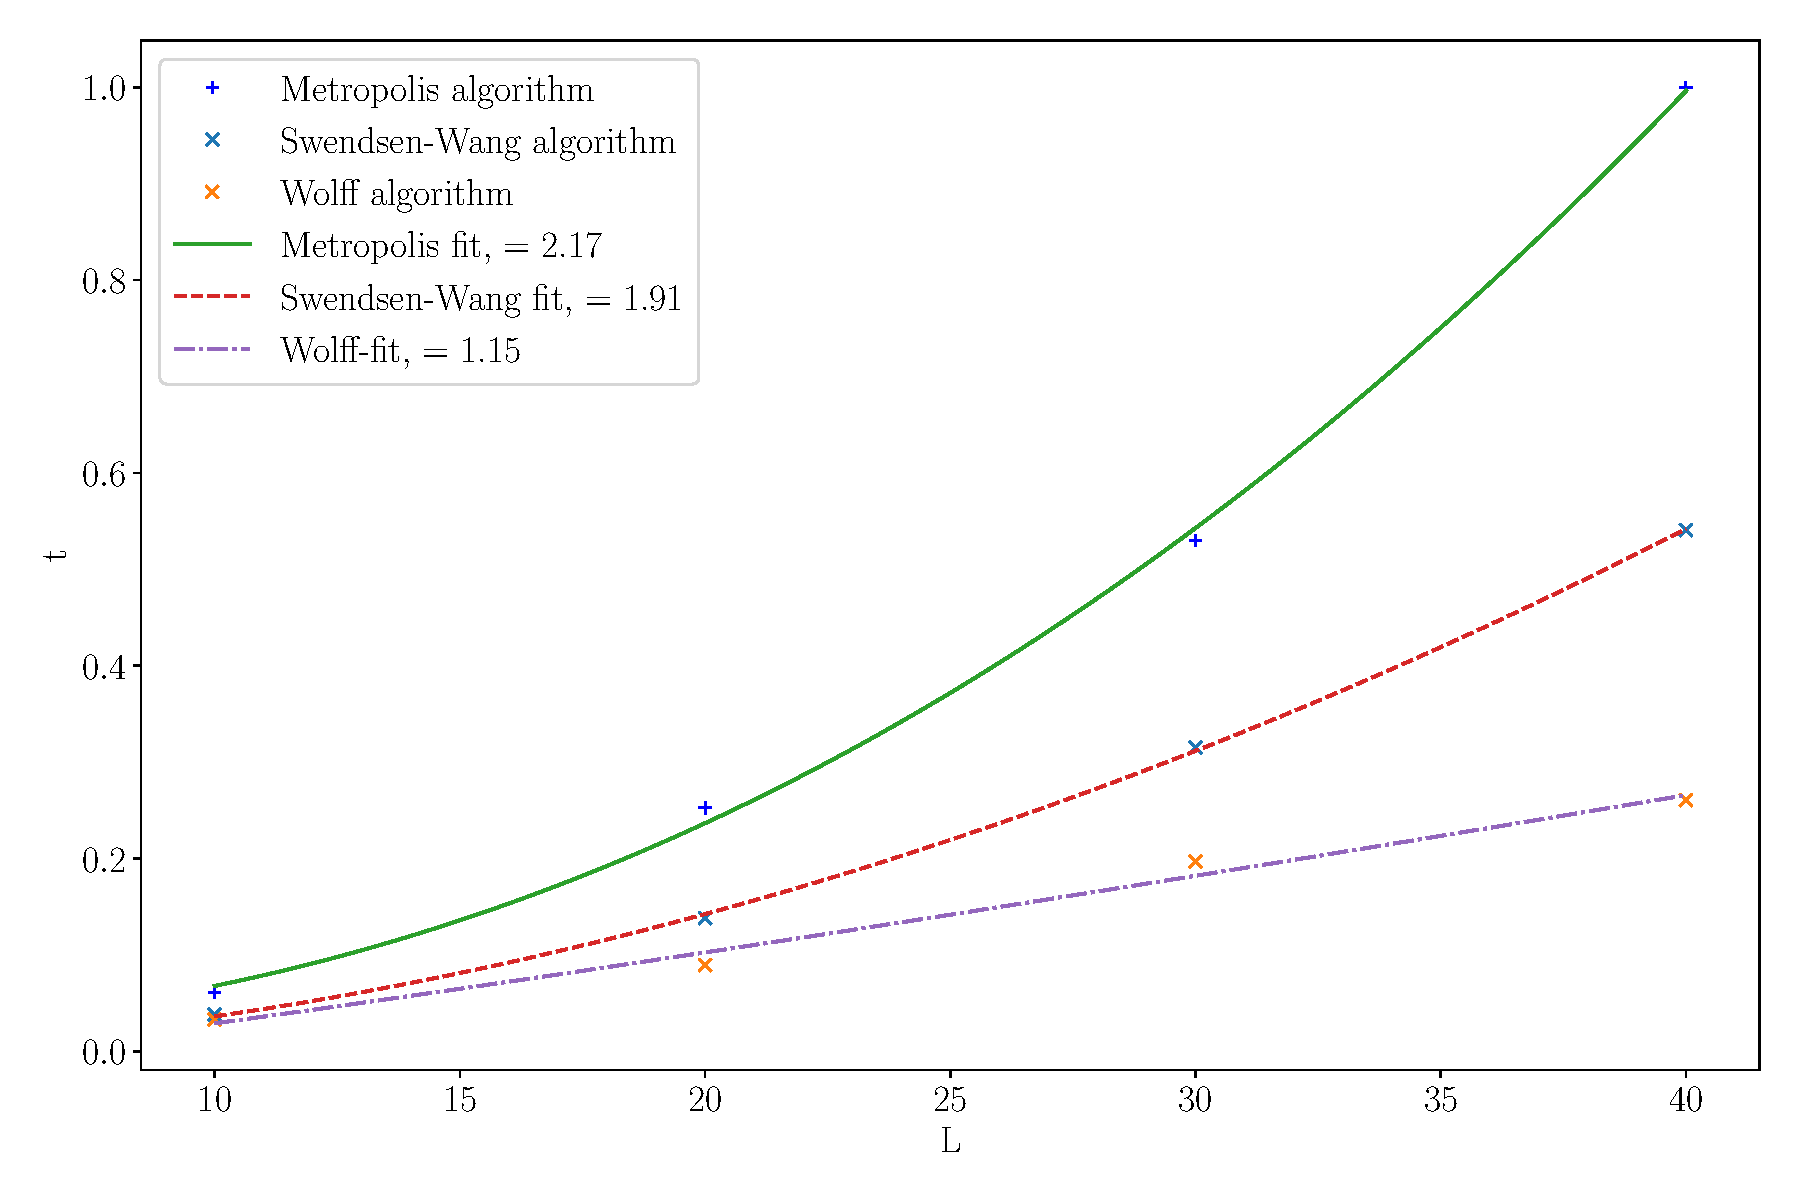
\includegraphics[scale = 0.35]{sim_performancewith_coeff.pdf}
    \caption{Simulation performance (normalzied run time) for Metropolis, SW and Wolff algorithm against different lattice size.}
    \label{fig:plot29}
\end{figure}

This view on the simulation performance is still omitting the fact that the Wolff algorithm has a much smaller dynamical critical exponent than the SW, which is better over MA. This means that the simulation can be run for a shorter time period to determine the physical quantities and thus makes the Wolff as well as SW algorithm much more efficient over MA.

\subsection{Clusters for Wolff and SW algorithms}
The view of how cluster looks in SW and Wolff algorithm is shown in the figure \ref{fig:cluster_sw} and \ref{fig:cluster_wolff} respectively below critical temperature at T = 2.0. After the critical temperature, the cluster just appears like, it do appears in step 1 of both SW and wolff. 

\begin{figure}
    \centering
    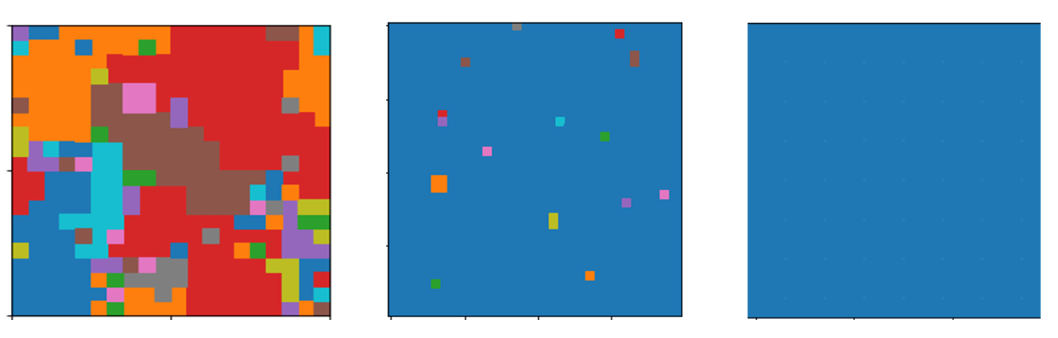
\includegraphics[width=0.75\linewidth]{SW algorithm.png}
    \caption{Cluster view for SW algorithm at different MC steps for L = 40 at T = 2.0}
    \label{fig:cluster_sw}
\end{figure}

\begin{figure}
    \centering
    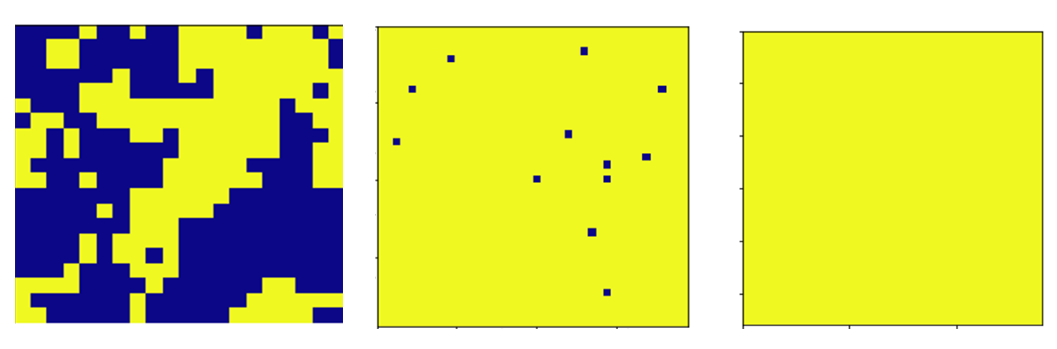
\includegraphics[width=0.75\linewidth]{wolff.png}
    \caption{Cluster identification for Wolff algorithm at different MC steps for L = 40, namely 100, 700, 1400 below critical temperature T = 2.0}
    \label{fig:cluster_wolff}
\end{figure}

\subsection{Geometric cluster}
The GCA as explained in theory part is applied on hard sphere model. The cluster is shown for three random mc steps at different time in figure \ref{fig:enternewgcalabel}. 

\begin{figure}
    \centering
    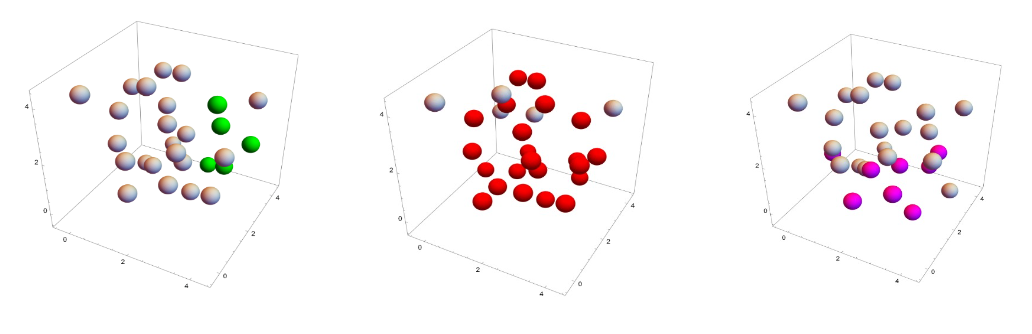
\includegraphics[width=0.8\linewidth]{GCA.png}
    \caption{GCA on Hard sphere in shown for three random MC steps. At every step some pivot is choosen and then they are flipped with respect to that pivot.}
    \label{fig:enternewgcalabel}
\end{figure}

\section{Conclusion}
The results presented in this report suggest that the simulation exhibits appropriate behavior with increasing system size, as all physical quantities appear to converge towards the limit of an infinite system. The critical exponent for magnetization closely matches the theoretical value for an infinite system. However, the critical exponents for other physical quantities display deviations from the infinite system limit, likely due to the finite dimensions of the system and the somewhat arbitrary selection of the fitting region. Further simulations with larger system sizes are necessary to validate these observations regarding system size. The selection of the fitting region was primarily based on visual inspection and lacks a solid theoretical foundation. Additional understanding of statistical methods is required to establish this theoretical background. The determination of the dynamical critical exponent aligns with existing literature. \\

The GCA, which is the application of cluster algorithms in off lattice models, is also presented. The project was aimed to understand how cluster algorithms are more efficient and general. This can have application to many models, where dynamics is hampered by critically slowing down. We both aimed to apply this for LJ potential, but unfortunately we are not able to because of the lack of time.  \\

\textbf{Cooperation}: In general, the workload was divided as evenly as possible. Initially, we both focused on developing various aspects of the Wolff algorithm, SW, and GCA, collaborating closely throughout the process. We would like to express our gratitude to Dr. Sunil Pratap Singh for providing us with the opportunity to work on this project during the course. Additionally, we extend our thanks to our friends for their assistance in running the code.






\newpage 
\clearpage
\printbibliography[title=\centering Bibliography]
\addcontentsline{toc}{chapter}{Bibliography} % Add Bibliography to the table of contents

\end{document}